% $  Id: validation.tex  $
% !TEX root = main.tex


%%
\section{Validation}
\label{sec:validation}

To validate the appropriateness of CollabIDE, we define two research questions
\begin{enumerate*}[label=(\arabic*)]
\item improve productivity, and
\item SPL
\end{enumerate*} 
To answer these questions, we conducted an empirical evaluation 
to measure how effective CollabIDE was at reducing overhead problems 
in both Distributed Software Development and Software Product Lines.

%%%%
\subsection{Experiment Design}

For each research question, we designed one experiment. In each experiment, we asked 
a group of developers to solve programming tasks using either CollabIDE or a 
conventional IDE following a set of instructions that aim to emulate the workflow that is carried out in each development model. The experiments differ in team sizes, the exercises that need to be solved and the workflow that must be followed to solve the exercises. For the Distributed Software Development experiment, there are groups developers that must each use JavaScript to accomplish their tasks and must also use version control periodically so that both team members code is updated with each other changes. For the Software Product Lines experiment, there are single developers that must use Java or JavaScript depending on the IDE being used to complete their tasks and must also use version control to manage the different product variants that are involved in these tasks. Two metrics are taken in each experiment, first, the percentage of completion of the total tasks assigned and second, the amount of time spent performing actions related to version control.

\authorcomment[missing]{NC}{Context, Research questions, analysis method, data collection method}
\begin{figure}[htbp]
  \centering
  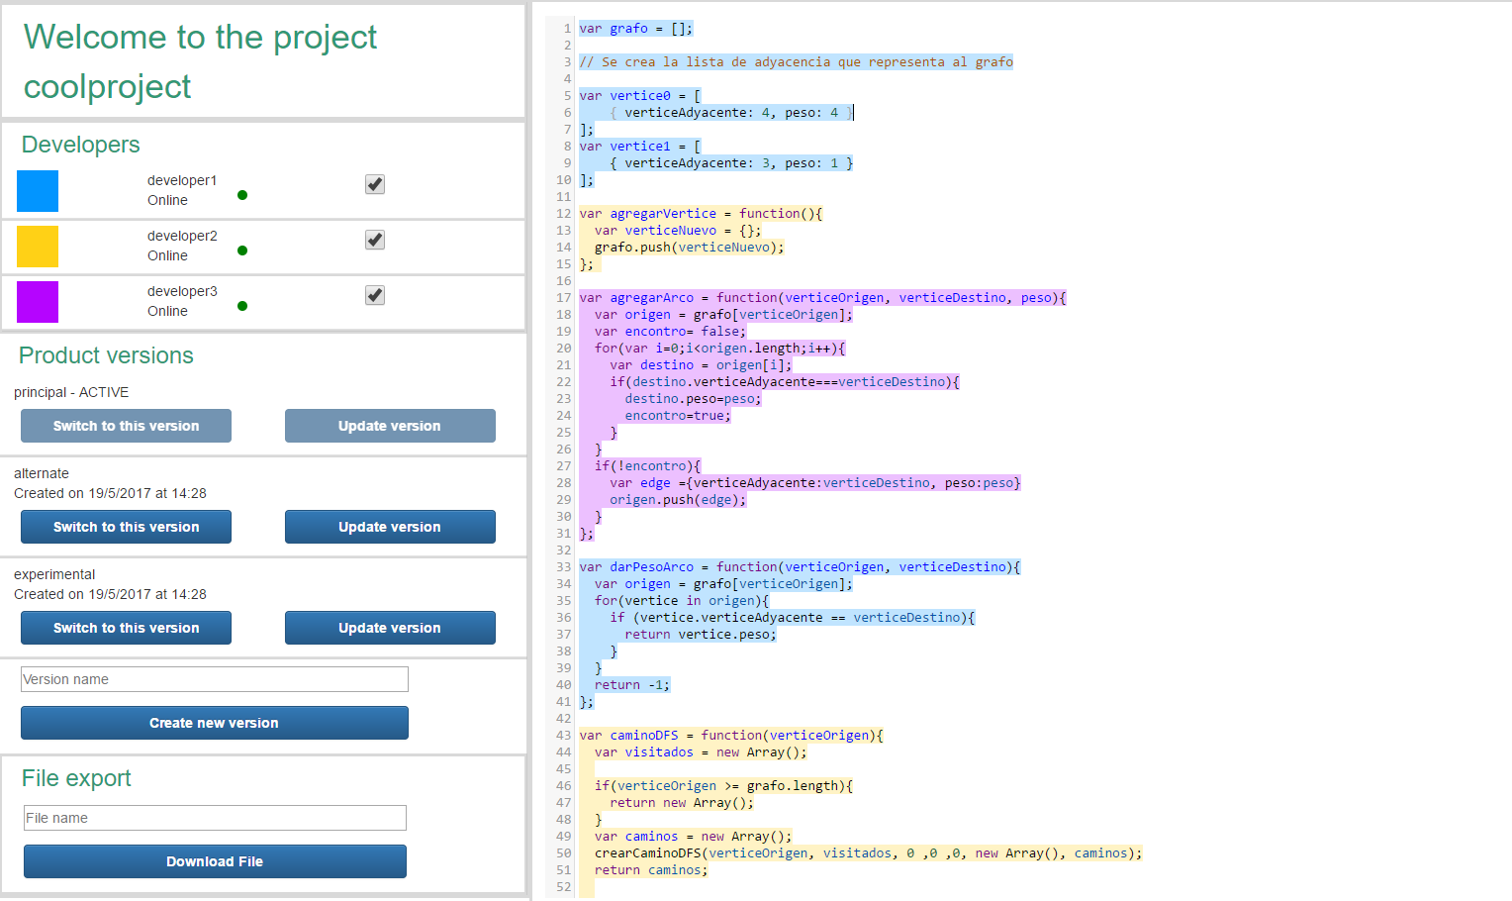
\includegraphics[width=0.7\textwidth]{img/fig1-collabIDEGeneral}
  \caption{CollabIDE tool}
  \label{fig:collabide}
\end{figure}

%%%%
\subsection{Experiment Setup}

Six developers were gathered for the Distributed Software Development experiment, then they were split into groups of two. Two groups would be using CollabIDE and the remaining group would be using Sublime Text in conjunction with git and github. The programming task for this experiment was to implement a set of common graph algorithms using only JavaScript. The participants were given a total of ninety minutes to accomplish this task. Each group was required to obtain their partner’s changes every fifteen minutes using their tools at hand.
In the Software Product Lines experiment, a different group of four developers was gathered. Two of them would be using CollabIDE and the other two would be using Eclipse in conjunction with git and github. In this case, the programming task was to implement a set of data structures with some basic functionality using JavaScript (CollabIDE) or Java (Eclipse). Each data structure also had to be a variant of a given base structure. These participants were also given ninety minutes to complete their task. In order to manage the different product variants, the participants were requested to use version control in each of their IDEs.


\authorcomment[missing]{NC}{Tools, exercise}
	

%%%%
\subsection{Results}

At the end of the experiment, the metrics showed that the developers which used CollabIDE obtained 
a higher completion percentage than those who used the other IDEs. The developers who used 
CollabIDE also spent significantly less time doing actions related to version control than the 
developers that used other IDEs.

%%%%
\subsection{Threads to Validity}



\endinput